\let\negmedspace\undefined
\let\negthickspace\undefined
\documentclass[journal,12pt,onecolumn]{article}
\usepackage{cite}
\usepackage{amsmath,amssymb,amsfonts,amsthm}
\usepackage{algorithmic}
\usepackage{graphicx}
\usepackage{textcomp}
\usepackage{xcolor}
\usepackage{txfonts}
\usepackage{listings}
\usepackage{enumitem}
\usepackage{mathtools}
\usepackage{gensymb}
\usepackage{comment}
\usepackage[breaklinks=true]{hyperref}
\usepackage{tkz-euclide} 
\usepackage{listings}
\usepackage{gvv}                                        
%\def\inputGnumericTable{}                                 
\usepackage[latin1]{inputenc}     
\usepackage{xparse}
\usepackage{color}                                            
\usepackage{array}                                            
\usepackage{longtable}                                       
\usepackage{calc}                                             
\usepackage{multirow}
\usepackage{multicol}
\usepackage{hhline}                                           
\usepackage{ifthen}                                           
\usepackage{lscape}
\usepackage{tabularx}
\usepackage{array}
\usepackage{float}
\usepackage{bm}
\newtheorem{theorem}{Theorem}[section]
\newtheorem{problem}{Problem}
\newtheorem{proposition}{Proposition}[section]
\newtheorem{lemma}{Lemma}[section]
\newtheorem{corollary}[theorem]{Corollary}
\newtheorem{example}{Example}[section]
\newtheorem{definition}[problem]{Definition}
\newcommand{\BEQA}{\begin{eqnarray}}
\newcommand{\EEQA}{\end{eqnarray}}
\usepackage{float}
%\newcommand{\define}{\stackrel{\triangle}{=}}
\theoremstyle{remark}
\usepackage{ circuitikz }
%\newtheorem{rem}{Remark}
% Marks the beginning of the document
\begin{document}

\title{CE - 2013}
\author{EE25BTECH11043 - Nishid Khandagre}
\date{}
\maketitle

\renewcommand{\thefigure}{\theenumi}
\renewcommand{\thetable}{\theenumi}

\section*{Q. 1 -- Q. 25 carry one mark each.}
\begin{enumerate}
    \item There is no value of $x$ that can simultaneously satisfy both the given equations. Therefore, find the 'least squares error' solution to the two equations, i.e., find the value of $x$ that minimizes the sum of squares of the errors in the two equations. \underline{\hspace{3cm}} (GATE-CE 2013)

    \begin{align}
    2x = 3 
    \end{align}
    \begin{align}
     4x = 1
    \end{align}

    \item What is the minimum number of multiplications involved in computing the matrix product $PQR$? Matrix $P$ has 4 rows and 2 columns, matrix $Q$ has 2 rows and 4 columns, and matrix $R$ has 4 rows and 1 column. \underline{\hspace{3cm}} (GATE-CE 2013)
    
    \item A 1-h rainfall of 10 cm magnitude at a station has a return period of 50 years. The probability that a 1-h rainfall of magnitude 10 cm or more will occur in each of two successive years is: (GATE-CE 2013)
    \begin{multicols}{4}
    \begin{enumerate}
        \item 0.04 
        \item 0.2 
        \item 0.02 
        \item 0.0004
    \end{enumerate}
    \end{multicols}
    
    \item Maximum possible value of Compacting Factor for fresh \brak{green} concrete is: (GATE-CE 2013)
    \begin{multicols}{4}
    \begin{enumerate}
        \item 0.5 
        \item 1.0 
        \item 1.5 
        \item 2.0
    \end{enumerate}
    \end{multicols}
    
    \item As per IS 800:2007, the cross-section in which the extreme fiber can reach the yield stress, but cannot develop the plastic moment of resistance due to failure by local buckling is classified as: (GATE-CE 2013)
    \begin{multicols}{2}
    \begin{enumerate}
        \item plastic section 
        \item compact section 
        \item semi-compact section 
        \item slender section
    \end{enumerate}
    \end{multicols}
    
    \item The creep strains are: (GATE-CE 2013)
    \begin{enumerate}
        \item caused due to dead loads only 
        \item caused due to live loads only 
        \item caused due to cyclic loads only 
        \item independent of loads
    \end{enumerate}
    
    \item As per IS 456:2000 for M20 grade concrete and plain bars in tension the design bond stress $\tau_{bd} = 1.2$ MPa. Further, IS 456:2000 permits this design bond stress value to be increased by 60\% for HSD bars. The stress in the HSD reinforcing steel bars in tension, $\sigma_s = 360$ MPa. Find the required development length, $L_d$, for HSD bars in terms of the bar diameter, $\phi$. \underline{\hspace{3cm}} (GATE-CE 2013)
    
    \item The 'plane section remains plane' assumption in bending theory implies: (GATE-CE 2013)
    \begin{enumerate}
        \item strain profile is linear 
        \item stress profile is linear 
        \item both strain and stress profiles are linear 
        \item shear deformations are neglected
    \end{enumerate}
    
    \item Two steel columns P (length $L$ and yield strength $f_y = 250$ MPa) and Q (length $2L$ and yield strength $f_y = 500$ MPa) have the same cross-sections and end-conditions. The ratio of buckling load of column P to that of column Q is: (GATE-CE 2013)
    \begin{multicols}{4}
    \begin{enumerate}
        \item 0.5 
        \item 1.0 
        \item 2.0 
        \item 4.0
    \end{enumerate}
    \end{multicols}
    
    \item The pin-jointed 2-D truss is loaded with a horizontal force of 15 kN at joint S and another 15 kN vertical force at joint U, as shown. Find the force in member RS (in kN) and report your answer taking tension as positive and compression as negative. \underline{\hspace{3cm}} (GATE-CE 2013)
    
    \begin{figure}[H]
    \centering
    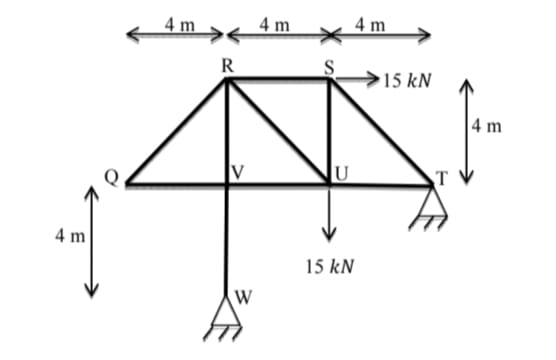
\includegraphics[width=0.7\columnwidth]{figs/image10.jpg}  
    \caption{}
    \label{fig:1}
    \end{figure}
    
    \item A symmetric I-section (with width of each flange = 50 mm, thickness of each flange = 10 mm, depth of web = 100 mm, and thickness of web = 10 mm) of steel is subjected to a shear force of 100 kN. Find the magnitude of the shear stress (in N/mm$^2$) in the web at its junction with the top flange. \underline{\hspace{3cm}} (GATE-CE 2013)
    
    \item In its natural condition, a soil sample has a mass of 1.980 kg and a volume of 0.001 m$^3$. After being completely dried in an oven, the mass of the sample is 1.800 kg. Specific gravity $G$ is 2.7. Unit weight of water is 10 kN/m$^3$. The degree of saturation of the soil is: (GATE-CE 2013)
    \begin{multicols}{4}
    \begin{enumerate}
        \item 0.65 
        \item 0.70 
        \item 0.54 
        \item 0.61
    \end{enumerate}
    \end{multicols}
    
    \item The ratio $N_f/N_d$ is known as shape factor, where $N_f$ is the number of flow lines and $N_d$ is the number of equipotential drops. Flow net is always drawn with a constant $b/a$ ratio, where $b$ and $a$ are distances between two consecutive flow lines and equipotential lines, respectively. Assuming that $b/a$ ratio remains the same, the shape factor of a flow net will change if the: (GATE-CE 2013)
    \begin{enumerate}
        \item upstream and downstream heads are interchanged 
        \item soil in the flow space is changed 
        \item dimensions of the flow space are changed 
        \item head difference causing the flow is changed
    \end{enumerate}
    
    \item Following statements are made on compacted soils, wherein DS stands for the soils compacted on dry side of optimum moisture content and WS stands for the soils compacted on wet side of optimum moisture content. Identify the incorrect statement: (GATE-CE 2013)
    \begin{enumerate}
        \item Soil structure is flocculated on DS and dispersed on WS. 
        \item Construction pore water pressure is low on DS and high on WS. 
        \item On drying, shrinkage is high on DS and low on WS. 
        \item On access to water, swelling is high on DS and low on WS.
    \end{enumerate}
    
    \item Four columns of a building are to be located within a plot size of 10 m $\times$ 10 m. The expected load on each column is 4000 kN. Allowable bearing capacity of the soil deposit is 100 kN/m$^2$. The type of foundation best suited is: (GATE-CE 2013)
    \begin{multicols}{2}
    \begin{enumerate}
        \item isolated footing 
        \item raft foundation 
        \item pile foundation 
        \item combined footing
    \end{enumerate}
    \end{multicols}
    
    \item For subcritical flow in an open channel, the control section for gradually varied flow profiles is: (GATE-CE 2013)
    \begin{enumerate}
        \item at the downstream end 
        \item at the upstream end 
        \item at both upstream and downstream ends 
        \item at any intermediate section
    \end{enumerate}
    
    \item Group-I contains dimensionless parameters and Group-II contains the ratios. (GATE-CE 2013)

    \begin{table}[H]
    \centering
    \begin{tabular}{|l|l|}
    \hline
    \textbf{Group-I} & \textbf{Group-II} \\
    \hline
    P. Mach Number & 1. Ratio of inertial force and gravitational force \\
    Q. Reynolds Number & 2. Ratio of fluid velocity and velocity of sound \\
    R. Weber Number & 3. Ratio of inertial force and viscous force \\
    S. Froude Number & 4. Ratio of inertial force and surface tension force \\
    \hline
    \end{tabular}
    \end{table}
    
    The correct match of dimensionless parameters in Group-I with ratios in Group-II is: (GATE-CE 2013)
    \begin{enumerate}
        \item P-3, Q-2, R-4, S-1 
        \item P-3, Q-4, R-2, S-1 
        \item P-2, Q-3, R-4, S-1 
        \item P-1, Q-3, R-2, S-4
    \end{enumerate}
    
    \item For a two-dimensional flow field, the stream function $\psi$ is given as $\psi = \frac{3}{2} \brak{y^2 - x^2}$. The magnitude of discharge occurring between the stream lines passing through points \brak{0,3} and \brak{3,4} is: (GATE-CE 2013)
    \begin{multicols}{4}
    \begin{enumerate}
        \item 6 
        \item 3 
        \item 1.5 
        \item 2
    \end{enumerate}
    \end{multicols}
    
    \item An isohyet is a line joining points of: (GATE-CE 2013)
    \begin{multicols}{2}
    \begin{enumerate}
        \item equal temperature 
        \item equal humidity 
        \item equal rainfall depth 
        \item equal evaporation
    \end{enumerate}
    \end{multicols}
    
    \item Some of the water quality parameters are measured by titrating a water sample with a titrant. Group-I gives a list of parameters and Group-II gives the list of titrants. (GATE-CE 2013)

    \begin{table}[H]
    \centering
    \begin{tabular}{|l|l|}
    \hline
    \textbf{Group-I} & \textbf{Group-II} \\
    \hline
    P. Alkalinity & 1. N/35.5 AgNO$_3$ \\
    Q. Hardness & 2. N/40 Na$_2$S$_2$O$_3$ \\
    R. Chloride & 3. N/50 H$_2$SO$_4$ \\
    S. Dissolved oxygen & 4. N/50 EDTA \\
    \hline
    \end{tabular}
    \end{table}
    
    The correct match of water quality parameters in Group-I with titrants in Group-II is:
    \begin{enumerate}
        \item P-1, Q-2, R-3, S-4 
        \item P-3, Q-4, R-1, S-2 
        \item P-2, Q-1, R-4, S-3 
        \item P-4, Q-3, R-2, S-1
    \end{enumerate}
    
    \item A water treatment plant is designed to treat 1 m$^3$/s of raw water. It has 14 sand filters. Surface area of each filter is 50 m$^2$. What is the loading rate (in m$^3$/day$\cdot$m$^2$) with two filters out of service for routine backwashing? \underline{\hspace{3cm}} (GATE-CE 2013)
    
    \item Select the strength parameter of concrete used in design of plain jointed cement concrete pavements from the following choices: (GATE-CE 2013)
    \begin{multicols}{2}
    \begin{enumerate}
        \item Tensile strength 
        \item Compressive strength 
        \item Flexural strength 
        \item Shear strength
    \end{enumerate}
    \end{multicols}
    
    \item It was observed that 150 vehicles crossed a particular location of a highway in a duration of 30 minutes. Assuming that vehicle arrival follows a negative exponential distribution, find out the number of time headways greater than 5 seconds in the above observation? \underline{\hspace{3cm}} (GATE-CE 2013)
    
    \item For two major roads with divided carriageway crossing at right angle, a full clover leaf interchange with four indirect ramps is provided. Following statements are made on turning movements of vehicles to all directions from both roads. Identify the correct statement: (GATE-CE 2013)
    \begin{enumerate}
        \item Merging from left is possible, but diverging to left is not possible. 
        \item Both merging from left and diverging to left are possible. 
        \item Merging from left is not possible, but diverging to left is possible. 
        \item Neither merging from left nor diverging to left is possible.
    \end{enumerate}
    
    \item The latitude and departure of a line $AB$ are +78 m and -45.1 m, respectively. The whole circle bearing of the line $AB$ is: (GATE-CE 2013)
    \begin{multicols}{4}
    \begin{enumerate}
        \item 30$\degree$ 
        \item 150$\degree$ 
        \item 210$\degree$ 
        \item 330$\degree$
    \end{enumerate}
    \end{multicols}

\section*{Q. 26 to Q. 55 carry two marks each.}

    \item The state of 2D-stress at a point is given by the following matrix of stresses:

    \begin{align}
    \myvec{
    \sigma_{xx} & \sigma_{xy} \\
    \sigma_{xy} & \sigma_{yy} }
    =
    \myvec{
    100 & 30 \\
    30 & 20 }
    \text{MPa}
    \end{align}

    What is the magnitude of maximum shear stress in MPa? (GATE-CE 2013)
    \begin{multicols}{4}
    \begin{enumerate}
        \item 50 
        \item 75 
        \item 100 
        \item 110
    \end{enumerate}
    \end{multicols}
    
    \item Find the magnitude of the error (correct to two decimal places) in the estimation of following integral using Simpson's $\frac{1}{3}$ Rule. Take the step length as 1. \underline{\hspace{3cm}} (GATE-CE 2013)

    \begin{align}
    \int_0^4 \brak{x^4 + 10} \, dx
    \end{align}
    
    \item The solution for 
    \begin{align}
    \int_0^{\pi/6} \cos^4 3\theta \sin^3 6\theta \, d\theta 
    \end{align}
    is: (GATE-CE 2013)
    \begin{multicols}{4}
    \begin{enumerate}
        \item 0 
        \item $\frac{1}{15}$ 
        \item 1 
        \item $\frac{8}{3}$
    \end{enumerate}
    \end{multicols}
    
    \item Find the value of $\lambda$ such that the function $f(x)$ is a valid probability density function. \underline{\hspace{3cm}} (GATE-CE 2013)
    \begin{align}
    f(x) = \lambda \brak{x-1}\brak
    {2-x} \quad \text{for } 1 \leq x \leq 2
    \end{align}
    \begin{align}
    = 0 \quad \text{otherwise}
    \end{align}
    
    \item Laplace equation for water flow in soils is given below.
    
    \begin{align}
    \frac{\partial^2 H}{\partial x^2} + \frac{\partial^2 H}{\partial y^2} + \frac{\partial^2 H}{\partial z^2} = 0
    \end{align}
    
    Head $H$ does not vary in $y$ and $z$ directions.\\
    Boundary conditions are: at $x = 0$, $H = 5$, and $\frac{dH}{dx} = -1$.\\
    What is the value of $H$ at $x = 1.2$? \underline{\hspace{3cm}} (GATE-CE 2013)
    
    \item All members in the rigid-jointed frame shown are prismatic and have the same flexural stiffness EI. Find the magnitude of the bending moment at Q (in kNm) due to the given loading. \underline{\hspace{3cm}} (GATE-CE 2013)
    
    \begin{figure}[H]
    \centering
    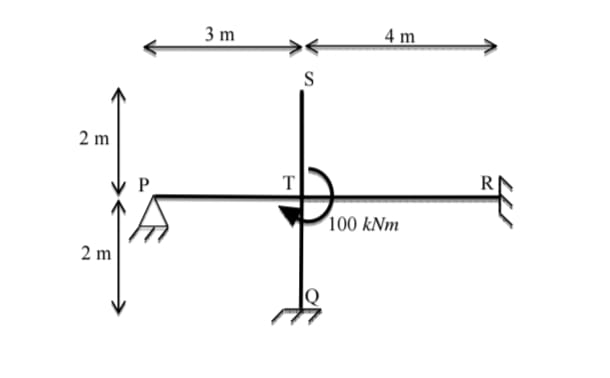
\includegraphics[width=0.7\columnwidth]{figs/image31.jpg}  
    \caption{}
    \label{fig:2}
    \end{figure}
    
    \item A uniform beam ($EI = \text{constant}$) $PQ$ in the form of a quarter-circle of radius $R$ is fixed at end $P$ and free at the end $Q$, where a load $W$ is applied as shown. The vertical downward displacement, $\delta_q$, at the loaded point $Q$ is given by: 
    $\delta_q = \beta \left( \frac{WR^3}{EI} \right)$. Find the value of $\beta$ (correct to 4-decimal places). \underline{\hspace{3cm}} (GATE-CE 2013)
    
    \begin{figure}[H]
    \centering
    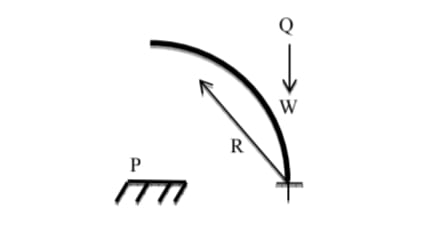
\includegraphics[width=0.7\columnwidth]{figs/image32.jpg}  
    \caption{}
    \label{fig:3}
    \end{figure}
    
    \item A uniform beam weighing 1800 N is supported at E and F by cable ABCD. Determine the tension (in N) in segment AB of this cable (correct to 1-decimal place). Assume the cables ABCD, BE and CF to be weightless. \underline{\hspace{3cm}} (GATE-CE 2013)
    
    \begin{figure}[H]
    \centering
    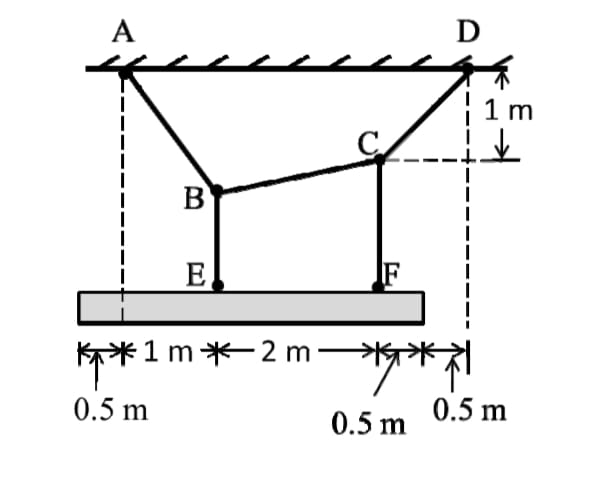
\includegraphics[width=0.7\columnwidth]{figs/image33.jpg}  
    \caption{}
    \label{fig:4}
    \end{figure}
    
    \item Beam PQRS has internal hinges in spans PQ and RS as shown. The beam may be subjected to a moving distributed vertical load of maximum intensity 4 kN/m of any length anywhere on the beam. The maximum absolute value of the shear force (in kN) that can occur due to this loading just to the right of support Q shall be: (GATE-CE 2013)
    \begin{figure}[H]
    \centering
    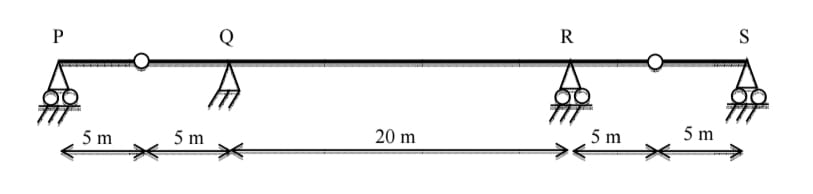
\includegraphics[width=0.7\columnwidth]{figs/image34.jpg}  
    \caption{}
    \label{fig:5}
    \end{figure}
    \begin{multicols}{4}
    \begin{enumerate}
        \item 30 
        \item 40 
        \item 45 
        \item 55
    \end{enumerate}
    \end{multicols}
    
    \item A rectangular concrete beam 250 mm wide and 600 mm deep is pre-stressed by means of 16 high tensile wires, each of 7 mm diameter, located at 200 mm from the bottom face of the beam at a given section. If the effective pre-stress in the wires is 700 MPa, what is the maximum sagging bending moment (in kNm) (correct to 1-decimal place) due to live load that this section of the beam can withstand without causing tensile stress at the bottom face of the beam? Neglect the effect of dead load of beam. \underline{\hspace{3cm}} (GATE-CE 2013)
    
    \item The soil profile below a lake with water level at elevation = 0 m and lake bottom at elevation = -10 m is shown in the figure, where $k$ is the permeability coefficient. A piezometer (stand pipe) installed in the sand layer shows a reading of +10 m elevation. Assume that the piezometric head is uniform in the sand layer. The quantity of water (in m$^3$/s) flowing into the lake from the sand layer through the silt layer per unit area of the lake bed is: (GATE-CE 2013)
    \begin{figure}[H]
    \centering
    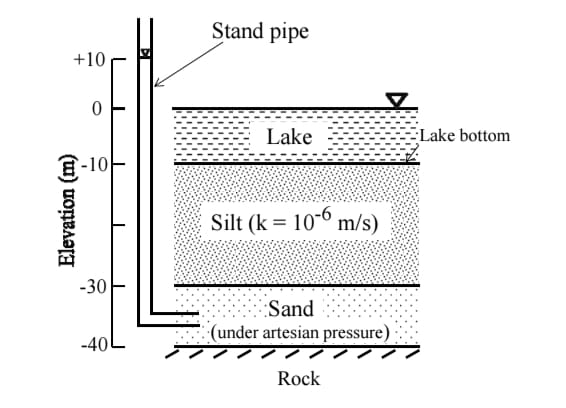
\includegraphics[width=0.7\columnwidth]{figs/image36.jpg}  
    \caption{}
    \label{fig:6}
    \end{figure}
    \begin{multicols}{4}
    \begin{enumerate}
        \item $1.5 \times 10^{-6}$ 
        \item $2.0 \times 10^{-6}$ 
        \item $1.0 \times 10^{-6}$ 
        \item $0.5 \times 10^{-6}$
    \end{enumerate}
    \end{multicols}
    
    \item The soil profile above the rock surface for a 25$\degree$ infinite slope is shown in the figure, where $s_u$ is the undrained shear strength and $\gamma_t$ is total unit weight. The slip will occur at a depth of: (GATE-CE 2013)
    \begin{figure}[H]
    \centering
    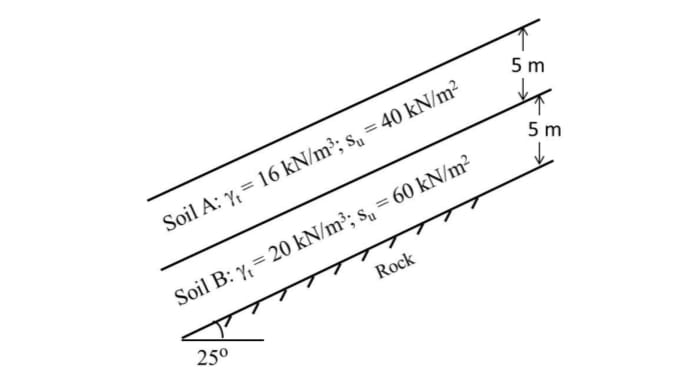
\includegraphics[width=0.7\columnwidth]{figs/image37.jpg}  
    \caption{}
    \label{fig:7}
    \end{figure}
    \begin{multicols}{4}
    \begin{enumerate}
        \item 8.83 m 
        \item 9.79 m 
        \item 7.83 m 
        \item 6.53 m
    \end{enumerate}
    \end{multicols}
    
    \item Two different soil types (Soil 1 and Soil 2) are used as backfill behind a retaining wall as shown in the figure, where $\gamma_t$ is total unit weight, and $c'$ and $\phi'$ are effective cohesion and effective angle of shearing resistance. The resultant active earth force per unit length (in kN/m) acting on the wall is: (GATE-CE 2013)
    \begin{figure}[H]
    \centering
    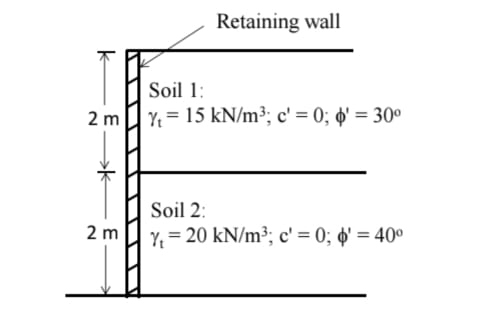
\includegraphics[width=0.7\columnwidth]{figs/image38.jpg}  
    \caption{}
    \label{fig:8}
    \end{figure}
    \begin{multicols}{4}
    \begin{enumerate}
        \item 31.7 
        \item 35.2 
        \item 51.8 
        \item 57.0
    \end{enumerate}
    \end{multicols}
    
    \item A 2 km long pipe of 0.2 m diameter connects two reservoirs. The difference between water levels in the reservoirs is 8 m. The Darcy-Weisbach friction factor of the pipe is 0.04. Accounting for frictional, entry and exit losses, the velocity in the pipe (in m/s) is: (GATE-CE 2013)
    \begin{multicols}{4}
    \begin{enumerate}
        \item 0.63 
        \item 0.35 
        \item 2.52 
        \item 1.25
    \end{enumerate}
    \end{multicols}
    
    \item The normal depth in a wide rectangular channel is increased by 10\%. The percentage increase in the discharge in the channel is: (GATE-CE 2013)
    \begin{multicols}{4}
    \begin{enumerate}
        \item 20.1 
        \item 15.4 
        \item 10.5 
        \item 17.2
    \end{enumerate}
    \end{multicols}
    
    \item The transplantation of rice requires 10 days and total depth of water required during transplantation is 48 cm. During transplantation, there is an effective rainfall (useful for irrigation) of 8 cm. The duty of irrigation water (in hectares/cumec) is: (GATE-CE 2013)
    \begin{multicols}{4}
    \begin{enumerate}
        \item 612 
        \item 216 
        \item 300 
        \item 108
    \end{enumerate}
    \end{multicols}
    
    \item A settling tank in a water treatment plant is designed for a surface overflow rate of 30 m$^3$/day$\cdot$m$^2$. Assume specific gravity of sediment particles = 2.65, density of water \brak{\rho} = 1000 kg/m$^3$, dynamic viscosity of water \brak{\mu} = 0.001 N$\cdot$s/m$^2$, and Stokes' law is valid. The approximate minimum size of particles that would be completely removed is: (GATE-CE 2013)
    \begin{multicols}{4}
    \begin{enumerate}
        \item 0.01 mm 
        \item 0.02 mm 
        \item 0.03 mm 
        \item 0.04 mm
    \end{enumerate}
    \end{multicols}
    
    \item A student began experiment for determination of 5-day, 20$\degree$C BOD on Monday. Since the 5th day fell on Saturday, the final DO readings were taken on next Monday. On calculation, BOD (i.e. 7 day, 20$\degree$C) was found to be 150 mg/L. What would be the 5-day, 20$\degree$C BOD (in mg/L)? Assume value of BOD rate constant $k$ at standard temperature of 20$\degree$C as 0.23/day (base $e$). \underline{\hspace{3cm}} (GATE-CE 2013)
    
    \item Elevation and temperature data for a place are tabulated below: (GATE-CE 2013)
    
    \begin{table}[H]
    \centering
    \begin{tabular}{|c|c|}
    \hline
    Elevation, m & Temperature, $\degree$C \\
    \hline
    4 & 21.25 \\
    444 & 15.70 \\
    \hline
    \end{tabular}
    \end{table}
    
    
    Based on the above data, lapse rate can be referred as:
    \begin{multicols}{2}
    \begin{enumerate}
        \item Super-adiabatic 
        \item Neutral 
        \item Sub-adiabatic 
        \item Inversion
    \end{enumerate}
    \end{multicols}
    
    \item The percent voids in mineral aggregate \brak{VMA} and percent air voids \brak{V_v} in a compacted cylindrical bituminous mix specimen are 15 and 4.5 respectively. The percent voids filled with bitumen \brak{VFB} for this specimen is: (GATE-CE 2013)
    \begin{multicols}{4}
    \begin{enumerate}
        \item 24 
        \item 30 
        \item 54 
        \item 70
    \end{enumerate}
    \end{multicols}
    
    \item Following bearings are observed while traversing with a compass. (GATE-CE 2013)
    
    \begin{table}[H]
    \centering
    \begin{tabular}{|l|c|c|}
    \hline
    Line & Fore Bearing & Back Bearing \\
    \hline
    AB & 126$\degree$45' & 308$\degree$00' \\
    BC & 49$\degree$15' & 227$\degree$30' \\
    CD & 340$\degree$30' & 161$\degree$45' \\
    DE & 258$\degree$30' & 78$\degree$30' \\
    EA & 212$\degree$30' & 31$\degree$45' \\
    \hline
    \end{tabular}
    \end{table}
    
    After applying the correction due to local attraction, the corrected fore bearing of line $BC$ will be:
    \begin{multicols}{4}
    \begin{enumerate}
        \item 48$\degree$15' 
        \item 50$\degree$15' 
        \item 49$\degree$45' 
        \item 48$\degree$45'
    \end{enumerate}
    \end{multicols}
    
    \item A theodolite is set up at station A and a 3 m long staff is held vertically at station B. The depression angle reading at 2.5 m marking on the staff is 6$\degree$10'. The horizontal distance between A and B is 2200 m. Height of instrument at station A is 1.1 m and R.L. of A is 880.88 m. Apply the curvature and refraction correction, and determine the R.L. of B (in m). \underline{\hspace{3cm}} (GATE-CE 2013)

    \section*{Common Data Questions}
    \textbf{Common Data for Questions 48 and 49}

    
    A propped cantilever made of a primatic steel beam is subjected to a concentrated load P at mid span as shown.
    \begin{figure}[H]
    \centering
    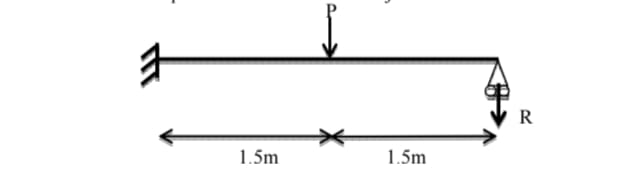
\includegraphics[width=0.7\columnwidth]{figs/image48.jpg}  
    \caption{}
    \label{fig:9}
    \end{figure}
    
    \item If load P=80 kN, find the reaction R (in kN) (correct to 1-decimal place) using elastic analysis. \underline{\hspace{3cm}} (GATE-CE 2013)
    
    \item If the magnitude of load P is increased till collapse and the plastic moment carrying capacity of steel beam section is 90 kNm, determine reaction R (in kN) (correct to 1-decimal place) using plastic analysis. \underline{\hspace{3cm}} (GATE-CE 2013)


    \textbf{Common Data for Questions 50 and 51:}

    
    For a portion of national highway where a descending gradient of 1 in 25 meets with an ascending gradient of 1 in 20, a valley curve needs to be designed for a vehicle travelling at 90 kmph based on the following conditions

    1) headlight sight distance equalto the stopping sight distance SSD of a level terrain considering length of valley curve$>$SSD.
    
    2) comfort condition with allowablerate of change of centrifugal acceleration=0.5 m/sec$^3$.

    Assume total reaction time=2.5 seconds, coefficient of longitudinal friction of the pavement=0.35, height of head light of the vehicle=0.75 m, andbeam angle=1$\degree$

    
    \item What is the length of valley curve (in m) based on the head light sight distance condition? \underline{\hspace{3cm}} (GATE-CE 2013)
    
    \item What is the length of valley curve (in m) based on the comfort condition? \underline{\hspace{3cm}} (GATE-CE 2013)


\section*{Linked Answer Questions}
    
\textbf{Statement for Linked Answer Question 52 and 53:}


A multistory building with a basement is to be constructed. The top 4 m consists of loose silt, below which dense sand layer is present up to a great depth. Ground water table is at the surface. The foundation consists of the basement slab of 6 m width which will rest on the top of dense sand as shown in the figure. For dense sand, saturated unit weight = 20 kN/m$^3$, and bearing capacity factors $N_q = 40$ and $N_\gamma = 45$. For loose silt, saturated unit weight = 18 kN/m$^3$, $N_q = 15$ and $N_\gamma = 20$. Effective cohesion $c'$ is zero for both soils. Unit weight of water is 10 kN/m$^3$. Neglect shape factor and depth factor.

Average elastic modulus E and Poison's ratio $\micro$ of dense sand is 60 x 10$^3$kN/m$^2$ and 0.3 respectively.

 \begin{figure}[H]
    \centering
    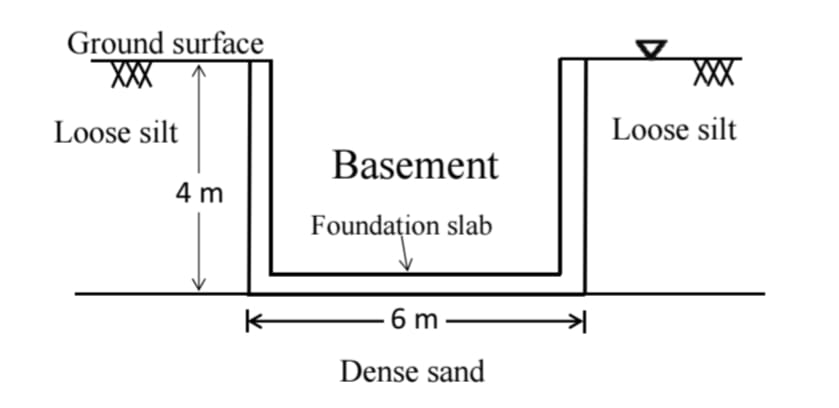
\includegraphics[width=0.7\columnwidth]{figs/image52.jpg}  
    \caption{}
    \label{fig:10}
    \end{figure}

    
    \item Using factor of safety = 3, the net safe bearing capacity (in kN/m$^2$) of the foundation is: (GATE-CE 2013)
    \begin{multicols}{4}
    \begin{enumerate}
        \item 610 
        \item 320 
        \item 983 
        \item 693
    \end{enumerate}
    \end{multicols}
    
    \item The foundation slab is subjected to vertical downward stresses equal to net safe bearing capacity derived in the above question. Using influence factor $I_f$ = 2.0, and neglecting embedment depth and rigidity corrections, the immediate settlement of the dense sand layer will be: (GATE-CE 2013)
    \begin{multicols}{4}
    \begin{enumerate}
        \item 58 mm 
        \item 111 mm 
        \item 126 mm 
        \item 179 mm
    \end{enumerate}
    \end{multicols}

    \textbf{Statement for Linked Answer Questions 54 and 55:}

    At a station, Storm I of 5 hour duration with intensity 2 cm/h resulted in a runoff of 4 cm and Storm II of 8 hour duration resulted in a runoff of 8.4 cm. Assume that the $\phi$-index is the same for both the storms.
    
    \item The $\phi$-index (in cm/h) is: (GATE-CE 2013)
    \begin{multicols}{4}
    \begin{enumerate}
        \item 1.2 
        \item 1.0 
        \item 1.6 
        \item 1.4
    \end{enumerate}
    \end{multicols}
    
    \item The intensity of storm II (in cm/h) is: (GATE-CE 2013)
    \begin{multicols}{4}
    \begin{enumerate}
        \item 2.00 
        \item 1.75 
        \item 1.50 
        \item 2.25
    \end{enumerate}
    \end{multicols}

\section*{General Aptitude (GA) Questions}
\textbf{Q. 56 -- Q. 60 carry one mark each.}
 
    \item A number is as much greater than 75 as it is smaller than 117. The number is: (GATE-CE 2013)
    \begin{multicols}{4}
    \begin{enumerate}
        \item 91 
        \item 93 
        \item 89 
        \item 96
    \end{enumerate}
    \end{multicols}
    
\item \underline{The professor}  \underline{ordered to}   \underline{the students to go}  \underline{out of the class}.

Which of the above underlined parts of the sentence is grammatically incorrect? (GATE-CE 2013)
    \begin{multicols}{4}
    \begin{enumerate}
        \item I 
        \item II 
        \item III 
        \item IV
    \end{enumerate}
    \end{multicols}
    
    \item Which of the following options is the closest in meaning to the word given below:
    Primeval (GATE-CE 2013)
    \begin{multicols}{4}
    \begin{enumerate}
        \item Modern 
        \item Historic 
        \item Primitive 
        \item Antique
    \end{enumerate}
    \end{multicols}
    
    \item Friendship, no matter how \underline{\hspace{1cm}} it is, has its limitations. (GATE-CE 2013)
    \begin{multicols}{4}
    \begin{enumerate}
        \item cordial 
        \item intimate 
        \item secret 
        \item pleasant
    \end{enumerate}
    \end{multicols}
    
    \item Select the pair that best expresses a relationship similar to that expressed in the pair:
    Medicine: Health  (GATE-CE 2013)
    \begin{multicols}{2}
    \begin{enumerate}
        \item Science: Experiment 
        \item Wealth: Peace 
        \item Education: Knowledge 
        \item Money: Happiness
    \end{enumerate}
    \end{multicols}

\textbf{Q. 61 to Q. 65 carry two marks each.}

    \item $X$ and $Y$ are two positive real numbers such that $2X + Y \leq 6$ and $X + 2Y \leq 8$. For which of the following values of $\brak{X, Y}$ the function $f\brak{X, Y} = 3X + 6Y$ will give maximum value? (GATE-CE 2013)
    \begin{multicols}{4}
    \begin{enumerate}
        \item \brak{4/3, 10/3} 
        \item \brak{8/3, 20/3} 
        \item \brak{8/3, 10/3} 
        \item \brak{4/3, 20/3}
    \end{enumerate}
    \end{multicols}
    
    \item If $|4X - 7| = 5$ then the values of $2|X| - |-X|$ is: (GATE-CE 2013)
    \begin{multicols}{4}
    \begin{enumerate}
        \item 2, 1/3 
        \item 1/2, 3 
        \item 3/2, 9 
        \item 2/3, 9
    \end{enumerate}
    \end{multicols}
    
    \item Following table provides figures in rupees on annual expenditure of a firm for two years - 2010 and 2011. (GATE-CE 2013)
    
    \begin{table}[H]
    \centering
    \begin{tabular}{|l|c|c|}
    \hline
    \textbf{Category} & \textbf{2010} & \textbf{2011} \\
    \hline
    Raw material & 5200 & 6240 \\
    Power \& fuel & 7000 & 9450 \\
    Salary \& wages & 9000 & 12600 \\
    Plant \& machinery & 20000 & 25000 \\
    Advertising & 15000 & 19500 \\
    Research \& Development & 22000 & 26400 \\
    \hline
    \end{tabular}
    \end{table}
    
    In 2011, which of the following two categories have registered increase by same percentage?
    \begin{enumerate}
        \item Raw material and Salary \& wages 
        \item Salary \& wages and Advertising 
        \item Power \& fuel and Advertising 
        \item Raw material and Research \& Development
    \end{enumerate}
    
    \item A firm is selling its product at Rs. 60 per unit. The total cost of production is Rs. 100 and firm is earning total profit of Rs. 500. Later, the total cost increased by 30\%. By what percentage the price should be increased to maintained the same profit level. (GATE-CE 2013)
    \begin{multicols}{4}
    \begin{enumerate}
        \item 5 
        \item 10 
        \item 15 
        \item 30
    \end{enumerate}
    \end{multicols}
    
    \item Abhishek is elder to Savar.
    Savar is younger to Anshul.
    
    Which of the given conclusions is logically valid and is inferred from the above statements? (GATE-CE 2013)
    \begin{enumerate}
        \item Abhishek is elder to Anshul 
        \item Anshul is elder to Abhishek 
        \item Abhishek and Anshul are of the same age 
        \item No conclusion follows
    \end{enumerate}
\end{enumerate}

\end{document}
